% $Id$
\documentclass[twocolumn,prd,nofootinbib]{revtex4}


\newcommand\ForInternalReference[1]{}
\newcommand\SkipForEarlyCirculation[1]{}
\newcommand\AddedResponse[1]{{\color{blue} {#1}}}
%\newcommand\SkipForEarlyCirculation[1]{#1}
\newcommand\SkipPP[1]{}
\usepackage{verbatim}
\usepackage{graphicx}
\usepackage{dcolumn}
\usepackage{bm}
\usepackage{color}
\usepackage{xspace}
\usepackage{url}
\usepackage{amsmath}
%\usepackage{adjustbox}
\usepackage{float}
\usepackage{multirow}
%
%
\usepackage{times}
%
%
%
\newcommand\optional[1]{}

%
\newcommand\E[1]{\left\langle #1\right\rangle}
\newcommand\qmstate[1]{\left|#1\right \rangle}
\newcommand\qmstateKet[1]{\left\langle#1\right|}
\newcommand\qmstateproduct[2]{\left\langle#1|#2\right\rangle}
\newcommand\qmoperatorelement[3]{\left\langle#1\left|#2\right|#3\right\rangle}
\newcommand\qmoperator[1]{{\bf #1}}
%
\newcommand\Y[1]{{{}_{#1}Y}}

\newcommand\lnL{ \ln {\cal L}}
\newcommand\lnLmarg{ \ln{\cal L}_{\rm marg}{}}
\newcommand\unit[1]{{\rm #1}}

\newcommand\rapidPEOrig{rapid\_pe1}
\newcommand\ILE{ILE}
\newcommand\editremark[1]{{\color{red} #1}}
%
%
%
\usepackage{color}
\definecolor{amber}{rgb}{1.0, 0.75, 0.0}
\definecolor{orange}{rgb}{1.0, 0.5, 0.0}
\definecolor{amaranth}{rgb}{0.9, 0.17, 0.31}
\def\fixme#1{\textcolor{red}{#1}}
\newcommand{\Richard}[1]{ {\color{blue}{#1}}}
\newcommand{\ros}[1]{ {\color{blue}{#1}}}
%

%

%
%
%
%
\graphicspath{{./figures/}}
\newcommand{\mc}{{\cal M}}
\newcommand{\Ms}{M_{\odot}}
\newcommand\LambdaTilde{\widetilde{\Lambda}}
\newcommand\DeltaLambdaTilde{\delta \widetilde{\Lambda}}
%
\def\ltsima{$\; \buildrel < \over \sim \;$}
\def\simlt{\lower.5ex\hbox{\ltsima}}
\def\gtsima{$\; \buildrel > \over \sim \;$}
\def\simgt{\lower.5ex\hbox{\gtsima}}

\newcommand\prx{Phys.~Rev.~X}
\def\aj{Astronomical Journal}                 %
\def\apj{Astrophysical Journal}                %
\def\apjl{Astrophysical Journal}             %
\def\pasj{PASJ}
\def\apjs{ApJS}              %
\def\mnras{MNRAS}            %
\def\prd{Phys.~Rev.~D}       %
\def\prl{Phys.~Rev.~Lett}    %
\def\cqg{Class.~Quant.~Grav.~}%
\def\araa{ARA\&A}             %
\def\nat{Nature}              %
\def\aap{A\&A}                %
\def\aapr{A\&A~Rev.~}    %
\def\pasp{PASP}    %
\def\sovast{Soviet Ast.}
%
%

\newcommand{\IMRPD}{\textsc{IMRPhenomD}\xspace}
\newcommand{\IMRPDT}{\textsc{IMRPhenomD\_NRTidal}\xspace}
\newcommand{\IMRP}{\textsc{IMRPhenomPv2}\xspace}
\newcommand{\SEOBP}{\textsc{SEOBNRv3}\xspace}
\newcommand{\SEOBA}{\textsc{SEOBNRv4}\xspace}
\newcommand{\SEOBAROM}{\textsc{SEOBNRv4\_ROM}\xspace}
\newcommand{\NRSur}{NRSur7dq2\xspace}
\newcommand{\TEOB}{SEOBNRv4T\xspace}
\newcommand{\Resum}{TEOBResumS\xspace}
\newcommand\RIFT{RIFT}
\newcommand{\Taylor}{TaylorF2\xspace}
\newcommand\PaperDetection{\underline{LVC-detect}\cite{DiscoveryPaper}}
\newcommand\PaperPE{\underline{LVC-PE}\cite{PEPaper}}
\newcommand\PaperTestGR{\underline{LVC-TestGR}\cite{TestingGRPaper}}
\newcommand\PaperPENRMethods{\underline{PE+NR-Methods}\cite{gwastro-PENR-Methods-Lange}}
\newcommand\PaperAstro{\underline{LVC-Astro}\cite{AstroPaper}}
\newcommand\PaperBurst{\underline{LVC-Burst}\cite{BurstPaper}}
\newcommand\PaperRates{\underline{LVC-Rates}\cite{RatesPaper}}
\newcommand\PaperStochastic{\underline{LVC-Stochastic}}
\newcommand\PaperSEOBNRvthree{\underline{LVC-SEOBNRv3}\cite{SEOBv3Paper}}

\def\RIT{Center for Computational Relativity and Gravitation, Rochester Institute of Technology, Rochester, New York 14623, USA}

\begin{document}

\title{Population Inference of Eccentric Binary Black Holes}
\author{M. Zeeshan}
\affiliation{\RIT}
\author{R. O'Shaughnessy}
\affiliation{\RIT}
\begin{abstract}
Yet to work. 
\end{abstract}
\maketitle

\section{Introduction}
The Advanced LIGO  \cite{2015CQGra..32g4001T}  and Virgo \cite{gw-detectors-Virgo-original-preferred}  ground-based gravitational wave (GW) detectors have
identified several coalescing compact binaries
\cite{DiscoveryPaper,LIGO-O1-BBH,2017PhRvL.118v1101A,LIGO-GW170814,LIGO-GW170608,LIGO-GW170817-bns}.  
%



\section{Methods}
\label{sec:methods}

The Binary Black Holes (BBHs) can be described by three intrinsic and seven extrinsic parameters. The intrinsic parameters: such as mass ($m_i$), spin $( \chi_i)$, and eccentricity $(e)$, are subject to the orbital evolution of the binary. The extrinsic parameters: orientation (orbital phase, polarization, and inclination), sky location (right ascension, declination), luminosity distance, and coalescence time depend on the observer.

{\color{red}Most of the eccentric binaries are driven by low mass events \cite{?}}. Therefore,  in this study, we  will consider modest masses $(1M_\odot-40M_\odot)$, non-spinning $(\chi_i = 0)$, and eccentric $(0-1)$ binaries. In addition, we will use mass ratio $q=m_1/m_2$ with condition $m_1>m_2$ and total mass $M=m_1+m_2$. 

\subsection{Hierarchical Bayesian Modeling}
\begin{itemize}
    \item We have N discrete detection.
    \item each detection has data $d_1,d_2,d_3,...,d_N$
    \item each data point $d_N$ has properties denoted by $\lambda_1,\lambda_2,...,\lambda_i$
    \item  $ \lambda_i$ are parameters such as mass, spin, eccentricity, and location.
    \item Each parameter has its uncertainty.
    \item This uncertainty is described by the probability of the data given the parameter value. We call it the likelihood function of one single event. $\mathcal{L}(\lambda) = p(d|\lambda)$
    \item the waveform gives the parameter value.
    \item waveform is a mathematical function.
    \item Once you have a likelihood function, you can use prior( usually it's uniform: which gives equal probability to each event) to find the posterior. $p(\lambda|d) \propto p(d|\lambda) p(\lambda)$  
    
\end{itemize}


\subsection{Population Inference}

\begin{itemize}
    \item We have the parameter estimation from RIFT or any other method. It will give us a distribution for each parameter, and we may take the mean value of it.
    \item Our first task is to find the likelihood function for the population parameters: such as mass and eccentricity.
    \item We denote population parameters with \\ $\Lambda \equiv  (\alpha, \mathcal{R}, m_{min}, m_{max}, e)$.
    \item uncertainty in $\Lambda$ is a likelihood which can be written as $\mathcal{L}(\Lambda)\equiv p(d_1,d_2,d_3,...,d_N|\Lambda)$
    \item By applying the Bayes theorem, we can turn above likelihood into posterior probability of a parameter.
\begin{equation}
\label{eq:Bayes}    
p(\Lambda|d_1,d_2,...,d_N)= \frac{p(\Lambda)p(d_1,d_2,...,d_N|\Lambda)}{p(d_1,d_2,...,d_N)}
\end{equation}

    \item where $p(\Lambda|d_1,d_2,d_3,...,d_N)$ is posterior, $p(\Lambda)$ is prior, $p(d_1,d_2,d_3,...,d_N)$ is normalization/evidence, and $p(d_1,d_2,d_3,...,d_N|\Lambda)$ is likelihood.
    \item We will use inhomogeneous Poisson Process scaled by rate $\mathcal{R} = \frac{dN}{dtdV_c}$ and parameterize by $\Lambda$ to find the likelihood  $\mathcal{L}(\mathcal{R},\Lambda)\equiv p(D|\mathcal{R},\Lambda)$ of an astrophysical population given the merger rate and parameter $\Lambda$. 
    {\color{red}I think these values of $\Lambda$ are provided by the power law model}. \\
\begin{equation}
\label{eq: likelihood}
\mathcal{L}(\mathcal{R},\Lambda) \propto e^{-\mu(\mathcal{R},\Lambda)}\prod_{n=1}^N\int d\lambda l_n(\lambda) \mathcal{R} p(\lambda|\Lambda)    
\end{equation}
        
    \item where $\mu(\mathcal{R},\Lambda)$ are the expected number of detections under the given population parametrization $\Lambda$ with overall rate $\mathcal{R}$. $l_n(\lambda)=p(d_n|\lambda)$ is the likelihood of the data $d_n$ given binary parameter.
    \item now we can find the posterior by Baye's theorem. \\
    $p(\mathcal{R},\Lambda)\propto p(\mathcal{R},\Lambda)  \mathcal{L}(\mathcal{R},\Lambda)$
    \item calculation of this posterior is computationally expensive, therefore, we will use MCMC method to find the posterior distribution.
    
\end{itemize}
\subsection{VT Estimation}
\begin{itemize}
    \item Estimation of VT (sensitivity of the LVK) only depend on the mass. For the sake of simplicity {\color{red}(physics reason)}, we consider only non-spinning, non-eccentric and nonprecessing BH Binaries. 
    \item Sources are detected if SNR is greater than 8.
    \item V is characteristic volume in which source can be detected by LVK. It is orientation averaged sensitive 3-volume.
\begin{equation}
\label{eq:volume}
V(\lambda) = \int P((<D(z))/D_n(\lambda))\frac{dV_c}{dz}\frac{dz}{1+z}
\end{equation}    
    \item where $D(z)$ is the luminosity distance for redshift z, $V_c$ is the comoving volume.

    \item to compute the $\mu(\mathcal{R},\Lambda)$, we use previously defined Volume in $Gpc^{-3}yr^{-1}$ and observing at this senstivity for the time $T$, the average number of detections would be as follows: \\
\begin{equation}
\label{eq:mu}
  \mu(\mathcal{R},\Lambda) = \int(VT)\lambda \mathcal{R}p(\lambda|\Lambda)d\lambda  
\end{equation}
    \item where $p(\lambda|\Lambda)$ is the probability density function for a random binary in the universe to have intrinsic paramter $\lambda$. Keep in mind that $\lambda$ is equal to all the 15 parameters of a binary.
\end{itemize}

\subsection{Power law Model}
The following is the power law model. We added the Gaussian eccentricity in it. 

\begin{align}
\label{eq:plawg}
p(m_1,m_2,e) = &C(\alpha,k_m,m_{min},m_{max},M_{max},e)  
\nonumber \\ & \frac{(m_2/m_1)^{k_m}m_1^{-\alpha}}{(m_1-m_{min})\sigma_e} 
\nonumber \\ &
\sqrt{\frac{2}{\pi}} e^{(-1/2)(e/\sigma_e)^2}
\end{align}
We use $k_m=0$, because GW networks are much more senstive to more massive BHs with $M\geq 200 M_\odot$

\begin{align}
\label{eq:plaw}
p(m_1,m_2,e) = &C(\alpha,m_{min},m_{max},M_{max},e)  
\nonumber \\ & \frac{m_1^{-\alpha}}{(m_1-m_{min})\sigma_e} 
\nonumber \\ &
\sqrt{\frac{2}{\pi}} e^{(-1/2)(e/\sigma_e)^2}
\end{align}

The probability density would be non zero only for the two following conditions.

\begin{itemize}
    \item $m_{min}\leq m_2 \leq m_1 \leq m_{max}$
    \item $m_1+m_2 \leq M_{max}$
\end{itemize}
Where $M_{max}$ depends on the detector (LVK)

   
\section{Inference of Synthetic BBH Population}
We have generated two distinct populations consistent of $100$ BBH by fixing the power law model parameter $\Lambda$ given in Eq. \ref{eq:plaw}. 
The parameters $\alpha=-2$, $m_{min}=10$, $m_{max}=50$ are same for both populations. The only difference between two generated populations is the dispersion of $\sigma_e$. The range for the first populations is $0<\sigma_e<0.5$ and for the second one is $0<\sigma_e<0.38$.
Furthermore, to make the comparison of the eccentric population with non-eccentric, we have created two more different populations by scaling already generated two populations by using the Eq. \ref{eq:scaling}. The Eq. \ref{eq:scaling} removes the eccentric component from the population, scales the masses and eventually we get non-eccentric population.
\begin{align}
\label{eq:scaling}
M^{ecc} = \frac{M}{(1-\frac{157}{24}e^2)^{3/5}}
\end{align}

\subsection{First Population: $0<\sigma_e<0.5$}
The following is the figure which shows the 

\begin{figure}
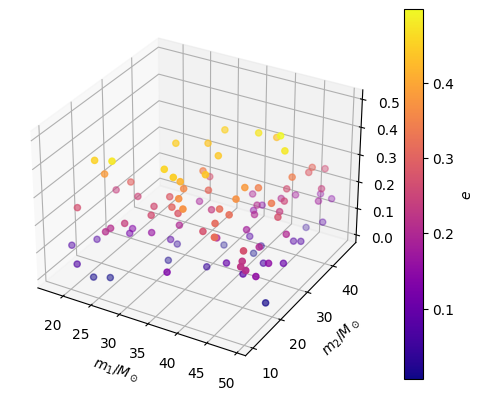
\includegraphics[width=0.45\textwidth]{paper/figures/pop3d05.png}
\caption{\label{fig:population05}\textbf{Synthetic Population of Eccentric BBHs}}
\end{figure}

\begin{figure}
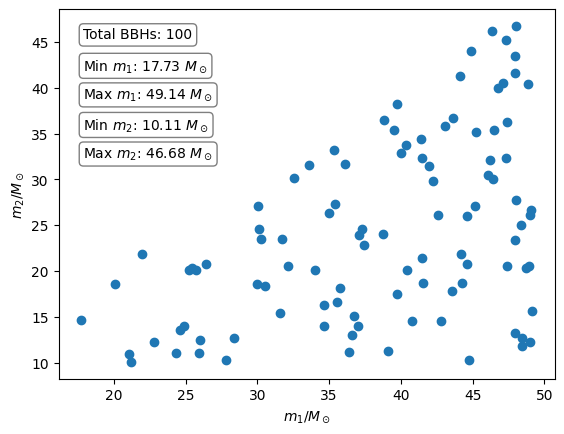
\includegraphics[width=0.45\textwidth]{paper/figures/pop2d05.png}
\caption{\label{fig:population05}\textbf{Synthetic Population of Eccentric BBHs}}
\end{figure}

\begin{figure}
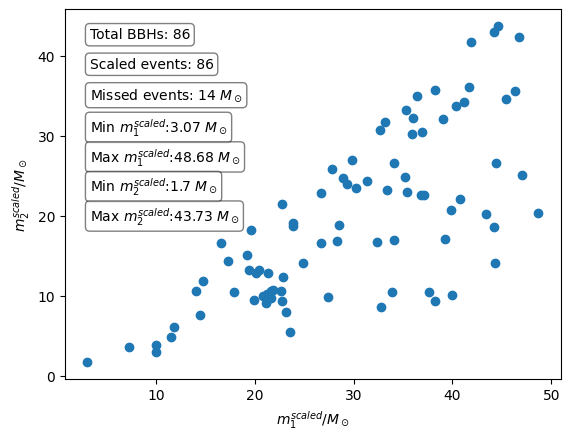
\includegraphics[width=0.45\textwidth]{paper/figures/pop2d05scl.png}
\caption{\label{fig:population05}\textbf{Synthetic Population of Eccentric BBHs}}
\end{figure}
\begin{figure}
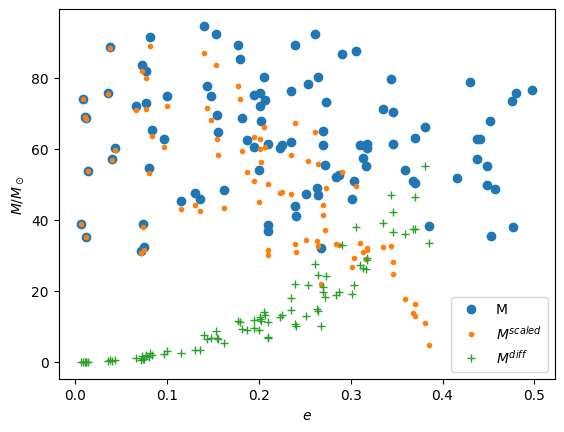
\includegraphics[width=0.45\textwidth]{paper/figures/pop2d05diff.png}
\caption{\label{fig:population05}\textbf{Synthetic Population of Eccentric BBHs}}
\end{figure}
\begin{figure}
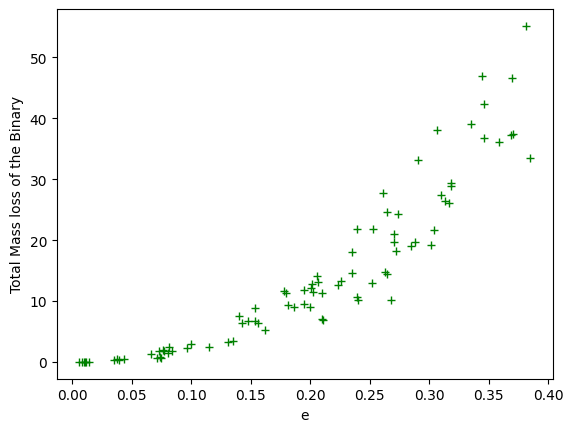
\includegraphics[width=0.45\textwidth]{paper/figures/massloss05.png}
\caption{\label{fig:population05}\textbf{Synthetic Population of Eccentric BBHs}}
\end{figure}





\subsection{Second Population: $0<\sigma_e<0.38$}



\begin{figure}
\includegraphics[width=0.45\textwidth]{paper/figures/massloss.png}
\caption{\label{fig:population05}\textbf{Synthetic Population of Eccentric BBHs}}
\end{figure}

\begin{figure}
\includegraphics[width=0.45\textwidth]{paper/figures/massloss.png}
\caption{\label{fig:population05}\textbf{Synthetic Population of Eccentric BBHs}}
\end{figure}

\begin{figure}
\includegraphics[width=0.45\textwidth]{paper/figures/massloss.png}
\caption{\label{fig:population05}\textbf{Synthetic Population of Eccentric BBHs}}
\end{figure}

\begin{figure}
\includegraphics[width=0.45\textwidth]{paper/figures/massloss.png}
\caption{\label{fig:population05}\textbf{Synthetic Population of Eccentric BBHs}}
\end{figure}

\begin{figure}
\includegraphics[width=0.45\textwidth]{paper/figures/massloss.png}
\caption{\label{fig:population05}\textbf{Synthetic Population of Eccentric BBHs}}
\end{figure}



% \begin{align} \label{eq:strain_mode}
% h(t,\vartheta,\phi;\bm{\lambda}) = 
% \sum_{\ell=2}^{\infty} \sum_{m=-\ell}^{\ell} \frac{D_{\rm ref}}{D} h^{\ell m}(t;\bm{\lambda}) \Y{-2}_{\ell m} \left(\vartheta, \phi \right) \, ,
% \end{align}


% \begin{widetext}
% \begin{align}
% \ln {\cal L}(\bm{\lambda}, \theta) 
% &= (D_{\rm ref}/D) \text{Re} \sum_k \sum_{\ell m}(F_k \Y{-2}_{\ell m})^* Q_{k,lm}(\bm{\lambda},t_k)\nonumber \\
% &   -\frac{(D_{\rm ref}/D)^2}{4}\sum_k \sum_{\ell m \ell' m'}
% \left[
% {
% |F_k|^2 [\Y{-2}_{\ell m}]^*\Y{-2}_{\ell'm'} U_{k,\ell m,\ell' m'}(\bm{\lambda})
% }
% % \right. \nonumber \\ & \left.
%  {
% +  \text{Re} \left( F_k^2 \Y{-2}_{\ell m} \Y{-2}_{\ell'm'} V_{k,\ell m,\ell'm'} \right)
% }
% \right]
% \label{eq:def:lnL:Decomposed}
% \end{align}
% \end{widetext}

% \begin{eqnarray}
% {\cal L}_{\rm margT} \equiv  \int {\cal L} \frac{dt}{T}
% \label{eq:lnL:tmarg}
% \end{eqnarray}












% \begin{table*}
% \begin{tabular}{lrr|ccccc|rr}
% Version & srate & modes & $\tau_{start}$ & $\tau_{setup}$ & $\tau_{ad}$ & $\tau_{it,like}$ &$\tau_{it,rest}$ &
% $\frac{T_{ILE}}{N_{eval}}$ & GPU \\  %\hline 
%   &   Hz & m & sec & sec & & $\mu$sec & $\mu$sec  &sec  & use  \%\\ \hline 
% % ~/parse_report.sh profile_nogpu_pcdev13.log | more
% CPU & 16384 & $\pm 2 $ & 20 & 2.4 &&540 & 20 &  690  \\ 
%        & 4096 & $\pm 2 $ &   20  &&&& 20 \\ \hline
% % ./parse_report.sh 20190130-profile_nogpu_HM_pcdev13.log  | more
% % /parse_report.sh ./profile_nogpu_HM_lowres_pcdev13.log 
% %    setup time: PrecomputeLikelihoodTerms, includes waveform generation. 
% %   evaluation: FactoredLogLikelihodTimeMarginalized Divide by actual number of calls, since not a block!
% %    
% CPU & 16384 & $\pm 2,\pm 1 $ & 20 & 1.5 && 680 & 20 &  1060  \\ 
%        & 4096 & $ \pm 2, \pm 1 $ &   20 &&&& 20  \\ \hline

%GPU (a) & 16384 & $\pm 2 $  & 20  & & && & 270 \\
%            & 4096 &$\pm 2 $  &  20 &  & & & & 45 \\ \hline

%GPU (b) & 16384 & $\pm 2$ & 20  & 1.8 & 1 & 0.85& 20 &28 & 15\\
%        & 4096 & $\pm 2$  & 20 & $1.2 $ &  1  & 0.75 & 20  & 25\\ \hline

% GPU (b) & 16384 & $\pm 2, \pm 1$ & 20 & 1 && 4.2 & 20  & 38  \\
%        & 4096 & $\pm 2, \pm 1$ & 20 & 1&& 2.5  & 20 & 35 & \\ \hline

% GPU (c) & 16384 & $\pm 2 $  & 20  &6  & & 18&  58&160 &  \\
%             & 4096 &$\pm 2 $  &  20 & 3.7 & & 11  & 58  & 140 & $\simeq 50$ \\
% \end{tabular}
% Compute node at LIGO-WA
% \caption{\label{tab:CostBreakdown}\textbf{Profiling performance: Binary black holes}: Evaluation costs for the
%   marginalized likelihood on default
%   hardware, for a two-mode system $(l,m)=\pm 2$ analyzing $T=8\unit{s}$ of data with a massive binary black hole
%   $m_1=35 M_\odot,M_2=30 M_\odot$.  The last column indicates peak GPU utilization.
% }
%\end{table*}










% \subsection{Binary black hole analysis}
% \label{sec:sub:BBHFull}

% \begin{figure*}

% 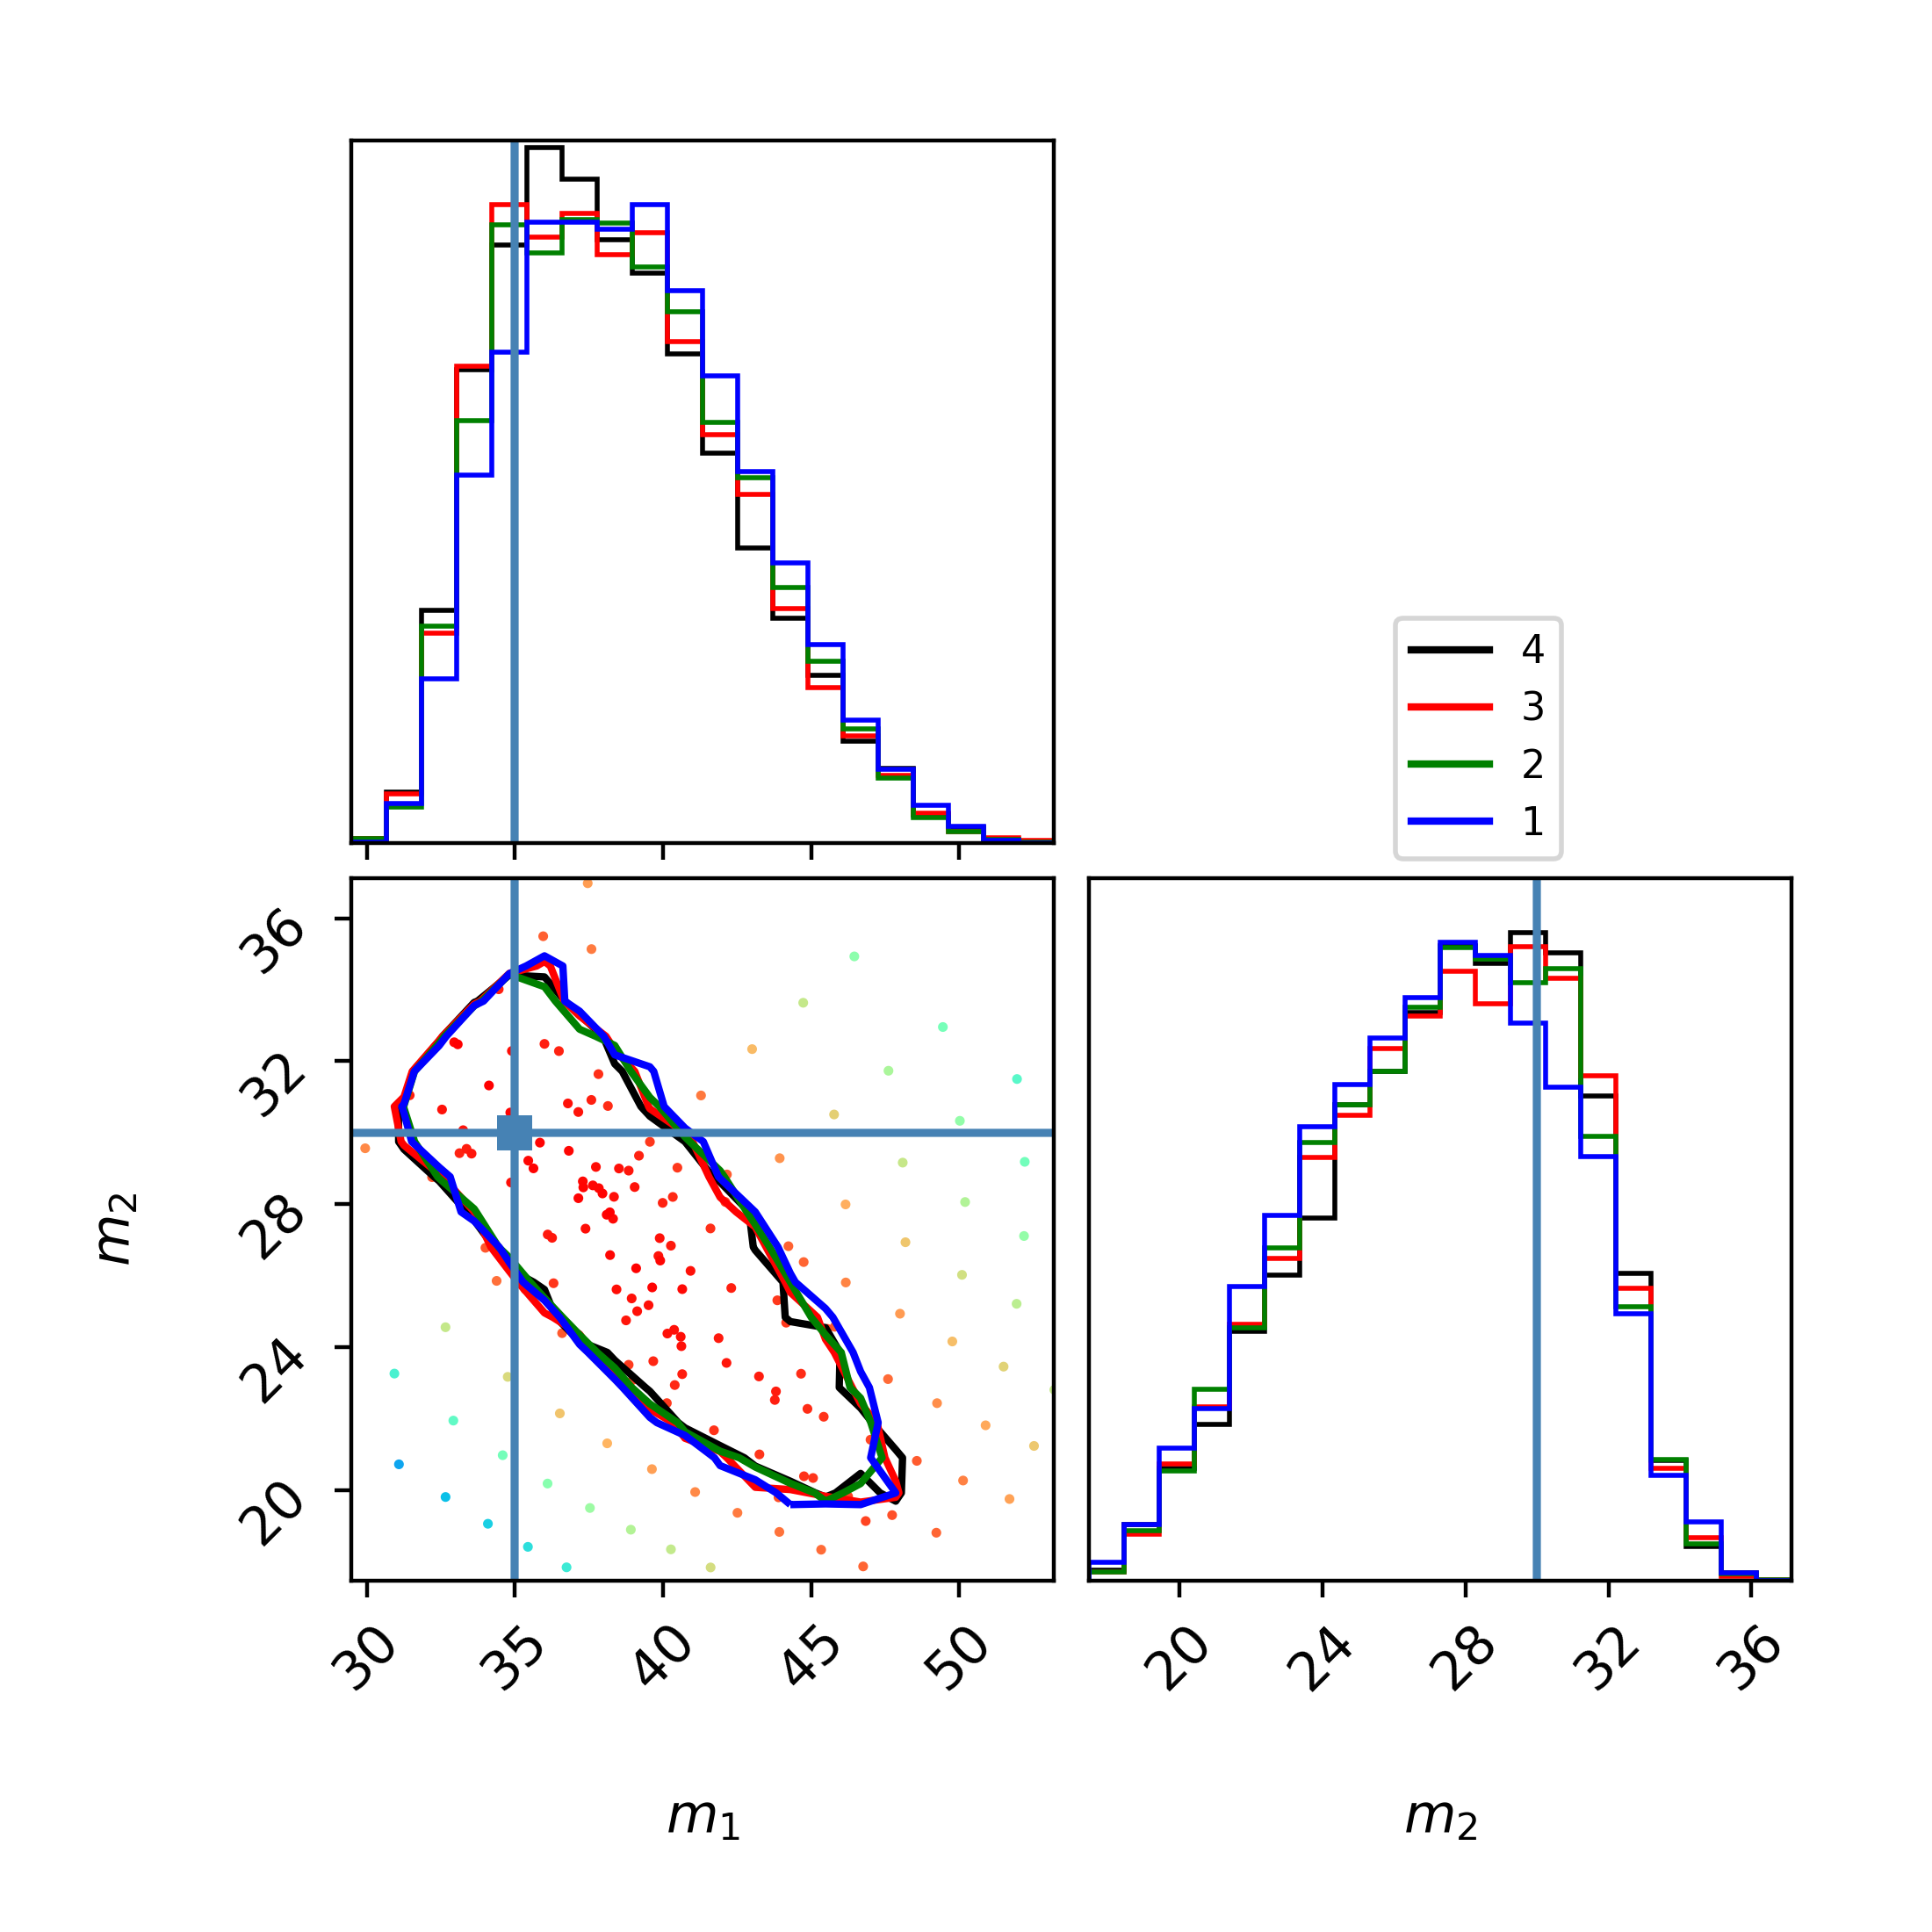
\includegraphics[width=0.45\textwidth]{figures/bbh_zerospin_m1_m2.png}
% 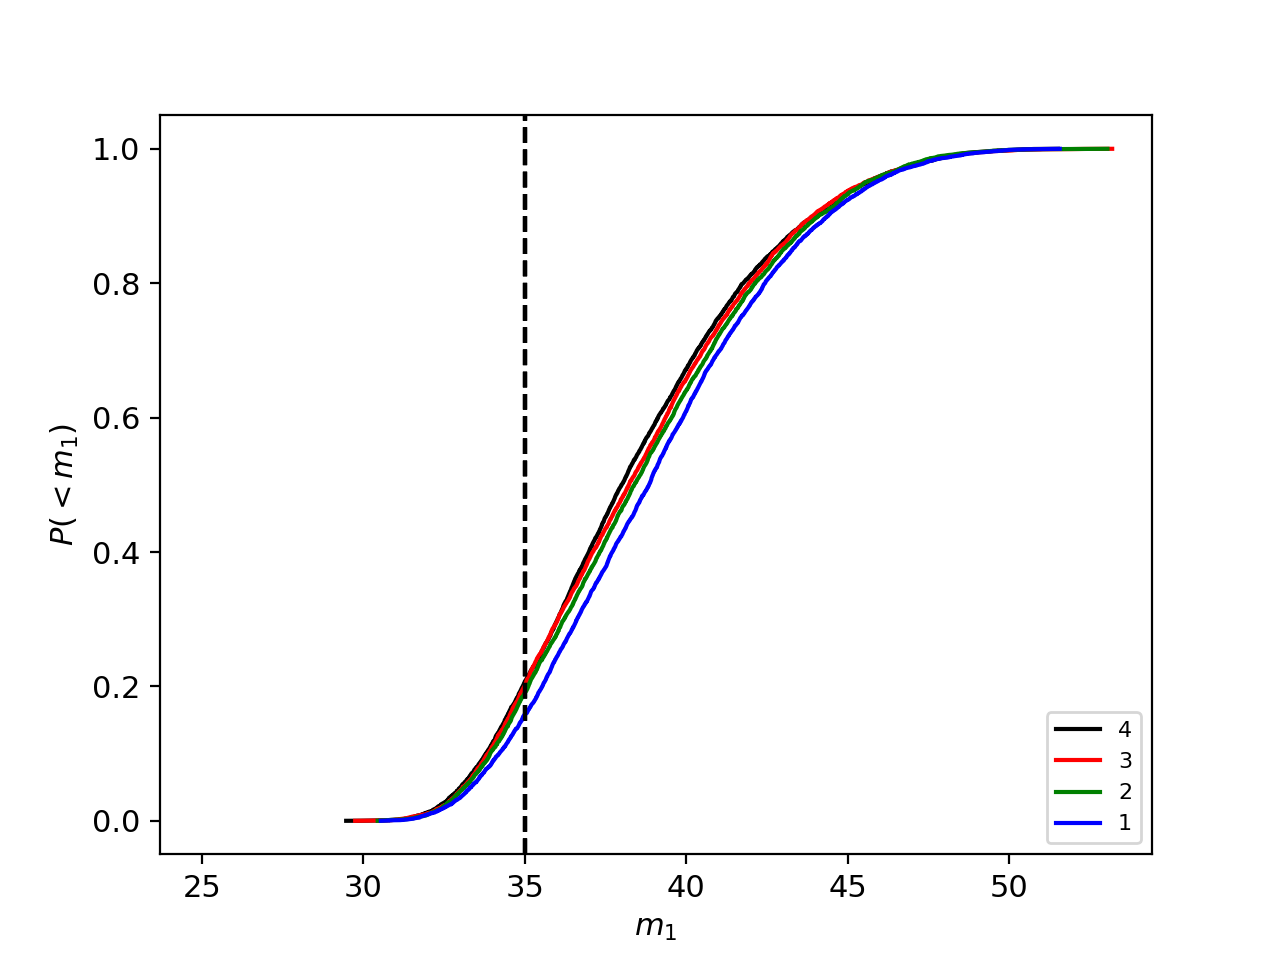
\includegraphics[width=0.45\textwidth]{figures/bbh_zerospin_m1_cum.png}
% % python plot_mean_variance.py --convergence-file 20190203-bbh-zerospin-batch_gpu_lowlatency_meanVar.dat  --output bbh_zerospin_lnL_meanVar
% 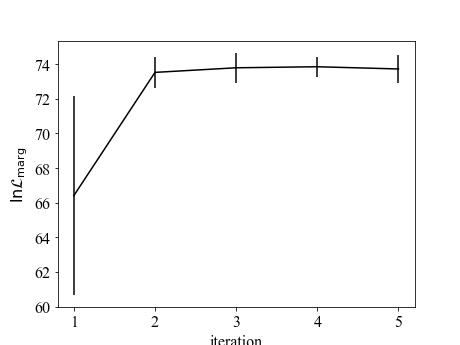
\includegraphics[width=0.45\textwidth]{figures/bbh_zerospin_lnL_meanVar.png}
% % python plot_convergence.py --convergence-file 20190203-bbh-zerospin-batch_gpu_lowlatency.dat
% 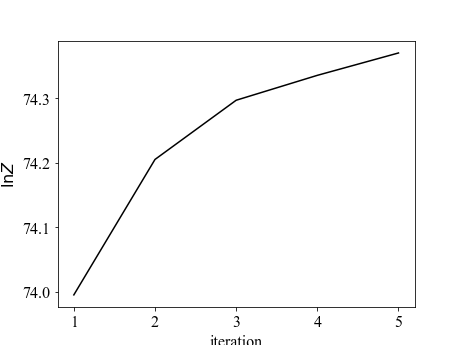
\includegraphics[width=0.45\textwidth]{figures/bbh_zerospin_lnL_converge.png}
% \caption{\label{fig:BBH:MultiIterate}\textbf{Convergence of BBH analysis: Zero spin}: Results for marginal posterior distributions
%   of our fiducial synthetic binary black hole.  Solid contours show credible intervals; solid one-dimensional distributions
%   show marginal CDFs and PDFs for the corresponding variable; and colored points indicate the location $\bm{\lambda}$ and
%   value of the underlying marginalized likelihood evaluations.   
% %The corresponding dotted curves show an analysis using   only the $m=\pm 2$ modes \editremark{perform both} 
% \emph{Left panel } Posterior distribution
%   over  $\mc$ and
%   $\delta=(m_1-m_2)/M$.    \emph{Right panel}: Marginal 1d CDFs of $\mc$, showing convergence.
% \emph{Bottom left}: Mean and variance of  \AddedResponse{the array $\ln{\cal L}_{\rm marg}(\bm{\lambda}_j)$  for
% $j=1,2,\ldots N_{\rm eval}$ indexing all candidate sets of intrinsic parameters $\bm{\lambda}_j$ performed in that iteration},  showing that after the
% first iteration the
% candidate points are consistent with the posterior (i.e., no proposed point has very low $\ln {\cal L}_{\rm marg}$).
% \emph{Bottom right panel}: The estimated evidence $Z = \int d\bm{\lambda} {\cal L}_{\rm marg}$ versus iteration number.  As systematic fitting error dominates our
% error budget, Monte Carlo error is not shown.
% }
% \end{figure*}


















\section{Conclusions}
\label{sec:conclude}
In Progress, 













\begin{acknowledgements}
We thank our anonymous referee for the helpful feedback.

\end{acknowledgements}


\appendix
In Progress,




%\bibstyle{unsrt}
\bibliography{paperexport,LIGO-publications}
\end{document}
